% vim: ts=4 sts=4 sw=4 tw=80
\chapter{Vim 脚本基础}
\label{chap:basic_vim_scripting}
\marginpar{141}

Vim 的一个最强大之处是允许高级用户通过编写脚本来增强 Vim 的功能. 通过脚本, 用
户几乎可以往 Vim 中添加任意功能, 而且很容易与其他用户分享.

这一章将会介绍编写 Vim 脚本的基础知识, 讨论的主题包括:
\begin{itemize}
    \item 编写语法高亮脚本
    \item 安装与使用脚本
    \item 不同类型的脚本
    \item 如何开发脚本
    \item Vim 脚本的基本语法
    \item 在 Vim 脚本中使用其他脚本语言
\end{itemize}

学习完这一章之后, 对于如何使用 Vim 脚本, 读者应该会有一个基本的概念, 而且有能
力写出一个简单的脚本, 从而为 Vim 添加新的功能.

\section{语法高亮方案}
\label{sec:syntax_color_schemes}

在许多程序员看来, 根据语法来高亮代码是 Vim 最重要的特性之一. 语法高亮不仅使代码
看起来更清晰, 还可以帮助用户发现编码错误. Vim 语法高亮系统所使用的脚本非常像
Vim 脚本, 但是语法高亮脚本定义的是颜色, 而不是功能. 在下面的一节里, 我们将会介
绍如何创建一个语法高亮方案.
\marginpar{142}

\subsection{第一个语法高亮文件}
\label{subsec:your_first_syntax_color_file}

简单来说, 语法高亮的关键是识别出文本中的特定单词与结构, 然后再给它们设置上对
应的颜色. 然而, 大部分情况下要稍微复杂一点, 因为语法高亮还需要识别上下文语境.
假设我们现在要语法高亮下面的代码:
\begin{vimcode}
/* if x equals y then return the value */
if (x == y)
  {
    return x;
  }
\end{vimcode}

如果我们仅仅是根据单词与符号来匹配, 那也可以得到一个相当不错的结果. 下面是具体
的配置命令 (每个选项的意义已经在第 \ref{chap:personalizing_vim} 章中进行了介
绍):
\begin{vimcode}
:syntax keyword myVars x y
:syntax match mySymbols "[{}();=]"
:syntax keyword myKeywords if return
:highlight myVars ctermfg=red guifg=red
:highlight mySymbols ctermfg=blue guifg=blue
:highlight myKeywords ctermfg=green guifg=green
\end{vimcode}

\begin{center}
    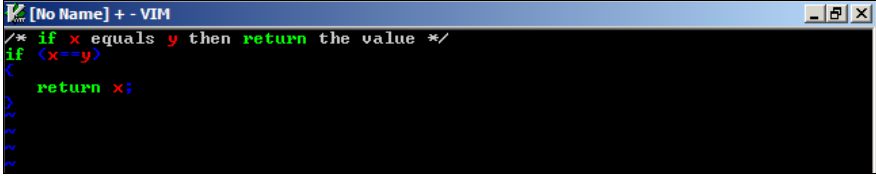
\includegraphics[scale=0.5]{./images/page142.png}
\end{center}

从上图中可以看到, 代码部分的高亮还不错, 可是注释语句却不令人满意. 这是因为我们
只是对单个单词进行匹配, 所以注释中的相同单词也会被匹配. 这种配置方法很难分辨出
代码与注释.
\marginpar{143}

那么, 我们可以从这个简单的例子里学习哪些东西呢? 那就是, 与高亮比起来, 更重要的
是要找到期望中的单词, 然后再给它们设置对应的颜色. 现在让我们增加一些上下文的信
息, 我们要把 \verb'/*' 与 \verb'*/' 之间的部分标记成注释, 然后再高亮其余的部
分. 代码部分被标记上颜色之后, 就不需要再上色了, 因此规则的顺序很重要. 具体的
配置代码是:
\begin{vimcode}
:syntax match myComments "/\*.*\*/"
:syntax keyword myVars x y
:syntax match mySymbols "[{}();=]"
:syntax keyword myKeywords if return
:highlight myVars ctermfg=red guifg=red
:highlight mySymbols ctermfg=blue guifg=blue
:highlight myKeywords ctermfg=green guifg=green
:highlight myComments ctermfg=yellow guifg=yellow
\end{vimcode}
最终的效果是:
\begin{center}
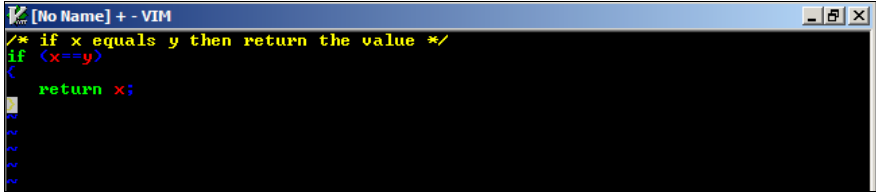
\includegraphics[scale=0.5]{./images/page143.png}
\end{center}

现在, 这段代码的高亮已经相当得体. 当然, 这只是一个小例子, 而且只用到了 Vim 语
法高亮的一小部分功能, 接下来, 我们将会介绍更多的内容.

\section{区域高亮}
\label{sec:syntax_regions}

在前面的例子中, 我们用的是选项 \texttt{match} 来选择注释语句. 在某些情况下,
我们很难创建一个适当的匹配语句, 这时候, 我们就需要用到其他一些更方便的做法.

在 Vim 中, 你可以选中一整个代码区, 然后再高亮它们, 为了选择一个代码区, 只需要
提供区域的开始与结束. 对于前面的例子, 如果使用区域高亮的话, 具体的命令是:
\begin{vimcode}
:syntax region myComments start=/\/\*/ end=/\*\//
\end{vimcode}
\marginpar{144}
有了这个命令, 很轻易就能匹配下面的任意一个注释块:
\begin{vimcode}
/* single line comment */
/*******************************
 *  multi line comments
 *******************************/
/* multi line comment
 */
\end{vimcode}

除了设置区域开始与结束, 选项 \texttt{region} 还可以做更多的事. 它还可以根据其
他语法规则来高亮区域内的某些代码. 我常做的一个操作是为函数注释设置几个关键词,
比如 \texttt{FIXME}, \texttt{OBSOLETE}, \texttt{TODO}, 等等, 这样, 我就可以把
代码写成:
\begin{vimcode}
/*  function: splitString()
 *  args    : string
 *  OBSOLETE
 */
function splitString(string) {
...
\end{vimcode}
剩下的工作, 就是创建一个关键词组:
\begin{vimcode}
:syntax keyword myKeywords OBSOLETE FIXME TODO
\end{vimcode}
现在, 我们需要修改命令 \texttt{region} 的设置, 以允许区域内包含其他语法元素,
修改后的命令是:
\begin{vimcode}
:syntax region myComments start=/\/\*/ end=\/\*\// contains=myKeywords
\end{vimcode}

如果需要在区域内包含多于一个的语法组, 只需要把它们写成列表的形式 (列表元素之间
用逗号分开), 再写到 \texttt{contains} 的后面.

\begin{warning}
    只有当开始与结束都在同一行时, 你才能告诉 Vim 这个区域是正确的, 方法是在
    命令 \texttt{syntax} 中添加一行选项. 如果没有这个选项, Vim 会在遇到开始时
    就开始高亮代码, 遇到结束时 (或者是文件的末尾) 停止.
\end{warning}
\marginpar{145}

在某些情况下, 用户可能希望在一个区域中嵌套另一个区域, 对于这种情况, 用户必须
把这项需求显式地告诉 Vim, 方法是在区域命令的末尾加上选项 \texttt{contained}:
\begin{vimcode}
:syntax region myComments start=/\/\*/ end=\/\*\// contains=myKeywords
contained
\end{vimcode}

在某些情况下, 一个代码块可以出现在代码中的任意一个位置, 当然, 用户不想针对每
一个代码块各写一个语法组, 这时候, 只需要把 \texttt{contains} 改成 \texttt{ALL}.

除了 \texttt{ALL}, 其他的关键词还包括:
\begin{itemize}
    \item \texttt{ALLBUT}: 如果它是列表的第一项, 那么列表中的其余项目在区域中
        都不会被高亮显示
    \item \texttt{CONTAINED}: 如果该项在列表中, 那么带有选项 \texttt{contained}
        的语法组就会在区域中被高亮显示
    \item \texttt{TOP}: 如果该项在列表中, 那么除了带有选项 \texttt{contained}
        的语法组, 其他所有的语法组都会被包含进来
\end{itemize}

有了上面的帮助, 用户就可以轻易地选择大范围的语法组, 而不用一个一个地把它们写下
来. 一个例子是选择除了 \texttt{myComments} 之外的所有语法组, 具体的命令是:
\begin{vimcode}
:syntax region myCodeblock start=/{/ end=/}/ contains=ALLBUT,myComments
\end{vimcode}

\begin{tips}
    如果用户知道某些语法组经常一起使用, 可以把它们放在一个簇 (cluster) 中:
    \texttt{:syntax cluster myCluster
    contains=myKeywords,mySymbols,myConditions}. 引用一个簇时可以在名字前加
    \verb'@': \texttt{:syntax region myComments start=}\verb'/\/\*/ end=/\*\//'
        \texttt{contains=@myCluster}.
\end{tips}

现在, 用户只需要把所有的配置命令都写到一个文件中, 再把这个文件放到
\texttt{VIMHOME} 的 \texttt{syntax} 子目录内. 文件的后缀名是 \texttt{.vim},
前缀名是文件所对应的编程语言源代码文件的后缀名, 比如 C 语言源代码文件的后缀名
是 \texttt{.c}, 那么它的语法文件就是 \texttt{c.vim}.

在前面的例子中, 所有语法组的名字都以 \texttt{my} 开始, 这是因为它所对应的编程
语言是 \texttt{my} (当然, 只是假设性的). 如果是 C 语言, 那么比较好的做法是
语法组的名字以 \texttt{c} 开始, 比如 \texttt{cKeywords}, \texttt{cConditions},
\texttt{cSymbols}, 等等).

继续前面的例子, 我们刚才说到 \texttt{my} 语法文件所对应的编程语言源代码文件
的后缀名是 \texttt{.my}, 为了简便起见, 我希望 Vim 把我的文件识别成具有文件类型
\texttt{my}.
\marginpar{146}

如果 Vim 无法识别用户正在编辑的文件, 那么就需要注册它们. 方法是在
\texttt{VIMHOME} 目录下的 \texttt{filetype.vim} 中添加几行. 如果该文件不存在,
可以手工创建. 对我的编程语言来说, 需要添加以下几行:
\begin{vimcode}
augroup filetypedetect
autocmd BufNewFile,BufRead *.my setfiletype my
augroup END
\end{vimcode}
上面的代码告诉 Vim 把两行 \texttt{augroup} 之间的所有内容都添加给自动命令组
\texttt{filetypedetect}. 这个命令组用于确定文件所拥有的文件类型.

在我们的例子中, 命令的功能是无论何时打开一个后缀为 \texttt{.my} 的文件, 就把
它的文件类型设置成 \texttt{my}. 如果用户还想区别其他文件类型, 还可以在两行
\texttt{augroup} 之间添加其他 \texttt{autocmd}.

注意, 如果 Vim 检查到我们正在编辑的文件的类型是 \texttt{my}, 它就会自动
查找匹配的语法文件, 它会在目录 \texttt{VIMHOME/syntax/} 内查找以文件类型名开始
的语法文件, 在这里就是 \texttt{my.vim}.

% TODO
% This is all you need to get started on creating your own syntax files that
% Vim can automatically load whenever you open one of your files.

\begin{warning}
    学习编写语法文件的最佳方法是阅读别人写的语法文件. 安装 Vim 后, 就已经安装
    了大量的语法文件, 涵盖了几乎所有常见的文件类型, 用户可以以它们为基础, 从
    而写出自己的语法文件.
\end{warning}

另一方面, 如果用户想要在已存在的语法文件中添加额外的识别, 有两种方法可以做到.
其中一种是找到那个文件, 然后添加自己的内容, 另外一种更好的办法是使用 Vim 的后
处理功能, 该功能可以覆盖 Vim 已经加载的脚本或语法文件. 第二种办法可以做到无论系统
上的脚本怎么更新, 都不用改动自己的部分, 因为它们已经和脚本隔离开了.

使用后处理器的秘诀是脚本文件的存放位置. 在用户的 \texttt{VIMHOME} 目录下, 有一
个子目录 \texttt{after} (如果不存在, 则手工创建). 无论 Vim 在何时查找脚本, 语
法文件, 或配色方案, 它都会在 \texttt{after} 子目录内查找同名的文件. 比如说, 如
果 Vim 找到了 \texttt{VIMHOME/syntax/c.vim}, 它就会接着查找
\texttt{VIMHOME/after/syntax/c.vim}, 看看是否有需要覆盖的地方. 这种情况同样
适用于从下面这些目录找到的脚本:
\marginpar{147}
\begin{itemize}
    \item \texttt{plugin}
    \item \texttt{ftplugin}
    \item \texttt{indent}
    \item \texttt{autoload}
    \item \texttt{syntax}
    \item \texttt{colors}
\end{itemize}
只要用户需要某个文件, 就可以把上面的任意一个目录放到 \texttt{after} 目录下,
如果 Vim 找到了文件, 就会使用它.

\subsection{配色方案与语法高亮}
\label{subsec:color_scheme_and_syntax_coloring}

在前面的例子中, 我们通过命令 \texttt{:syntax} 添加了用户自己的高亮色彩组. 这
使得用户对配色具有了完全的控制权, 但同时也限制了颜色的种类. 因此, 在其他地方
可能就不能使用这些颜色\footnote{Hence, it might not follow the colors defined
by the color scheme you use in the rest of Vim}.

一个更好的办法是使用 Vim 已经定义好了的色彩组, 这就把色彩定义与语法高亮分成了
两个部分. 通过这种方法, 无论在何时修改了配色方案, 语法高亮都会自动地更新.

下面的命令可以列出所有已经定义了的颜色:
\begin{vimcode}
:highlight
\end{vimcode}

\begin{warning}
    或者, 你还可以看一下配色方案文件, 这些文件存放在 \texttt{VIMHOME} 的
    \texttt{colors} 目录下.
\end{warning}

\section{使用脚本}
\label{sec:using_scripts}

每个人都会有一些特定的编辑器需求, 其中有些需求比较简单, 比如按键绑定, 而有一些
则比较复杂, 当然, Vim 不可能满足每个人的需要, 所以它提供了脚本供程序员扩展
Vim.
\marginpar{148}

但是如果用户不是个程序员, 或者没有时间自己开发脚本, 那又该怎么办呢? 这当然不是
个问题, Vim 是免费发布的, 因此有很多用户同样免费发布自己开发的脚本. 他们中的许
多人会把自己的脚本放到 \url{http://www.vim.org} 上供人免费下载, 其他用户很容易
就可以搜索到自己想要的脚本.

\subsection{脚本类型}
\label{subsec:script_types}

在 Vim 官网可以找到大量的脚本, 它们的功能各异, 有的很简单 (比如插入日期), 有的
则比较复杂 (比如 IDE 编程环境), 但是实际上, Vim 只能识别某几种预定义的脚本类型
组.

如果我们认真查看一下脚本类型, 就会发现它们可以分为两组, 第一组是全局插件组, 该
组包含的脚本会在 Vim 启动时, 或者是在用户执行某些特定的函数调用时补始化. 这种
脚本的典型例子包括为 Gvim 添加菜单, 为已经定义了的函数添加功能, 又或者是根据用
户的需要修改某些特性.

第二组是文件类型插件组. 该组包含的脚本和某个 (或某些) 特定的文件类型相关联, 只
有当相应类型的文件被打开或创建时, 才会加载脚本. 组内脚本的功能可以是为某个特定
的文件类型添加特性, 还可以是某些特定的工具. 比如, 为某种编程语言的编译操作定义
一个快捷键, 或者是在程序员编写的每一个函数上方添加一段注释. 组内的脚本还包括语
法高亮, 虽然和其他脚本相比, 语法高亮脚本的安装位置不太一样.

\subsection{安装脚本}
\label{subsec:installing_scripts}

下载脚本后, 它们的格式通常是下面三种之一:
\begin{itemize}
    \item 一个单一的 \texttt{.vim} 文件
    \item 一个压缩文件 (通常是 Zip 格式), 里面包含了一个或多个 \texttt{.vim}
        文件, 以及文档
    \item Vimball 格式, 一种 Vim 脚本安装文件
\end{itemize}

如果待安装的脚本仅仅是一个单一的脚本文件, 安装的方法是把它复制到
\texttt{VIMHOME/plugin} 目录下, 如果是和某种文件类型相关的脚本, 就复制到
\texttt{VIMHOME/ftplugin}.
\marginpar{149}
如果用户使用的是多用户操作系统, 只需要把它们安装在 Vim 安装目录 (而非
\texttt{VIMHOME}) 下面的同名子目录中, 就可以同时为所有的用户提供服务.

如果脚本被打包成压缩文件, 其安装方法就很难说清楚. 典型的安装方法是把压缩文件
复制到 \texttt{VIMHOME}, 然后再解压. 解压后, 压缩包中的文件会自动存放到对应的
目录内. 通常在压缩文件中都有一个 \texttt{README} 或 \texttt{INSTALL} 文件, 它
们详细介绍了脚本的安装方法.

\begin{warning}
    如果脚本是在 \url{http://www.vim.org} 上找到的, 那就同时也能找到脚本的安
    装方法.
\end{warning}

最后一种格式需要通过 Vimball 来安装, Vimball 是为 7 及以上版本的 Vim 而开发的.
Vim 接收若干个文件, 然后把它们组合成一个单一的 Vim 脚本归档文件, 文件的后缀名
是 \texttt{.vba}, 意思是 Vimball.

在开始使用 Vimball 之前, 得先安装 Vimball 脚本, 这个脚本用于读取与安装 Vimball
文件. 和其他脚本一样, 用户可以到 Vim 官网下载到该脚本.

\begin{warning}
    在 \url{http://www.vim.org/scripts/script.php?script_id=1502} 上可以下载
    到最新版的 Vimball.
\end{warning}

安装完 Vimball 脚本后, 就可以用它来安装其他 Vim 脚本.

假设用户现在有一个名为 \texttt{myscript.vba} 的 Vimball 文件, 为了安装它, 先
在 Vim 中打开该文件, 打开文件后, Vim 就会告诉用户如何安装
\texttt{myscript.vba}. 安装的方法通常是执行下面的命令:
\begin{vimcode}
:source %
\end{vimcode}
命令会把脚本安装到从选项 \texttt{runtimepath} 中找到的第一个目录内. 如果想修改
安装目录, 就把命令换成:
\begin{vimcode}
:UseVimball PATH
\end{vimcode}
\marginpar{150}
你需要把 \texttt{PATH} 替换成脚本的安装路径. 需要注意的是, 有些脚本只能安装在
特定的目录下, 否则的话, 脚本就不能正常工作.

有时候, 用户可能想在安装之前查看一下 Vimball 中包含的文件. Vim 提供了一个这样
的命令, 使用方法是在打开 Vimball 之后, 执行:
\begin{vimcode}
:VimballList
\end{vimcode}

查看后, 如果没什么问题, 就可以用 \texttt{:source} 或 \texttt{:UseVimball}
安装.

\subsection{卸载脚本}
\label{subsec:uninstalling_scripts}

通常来说, 不存在用于卸载脚本的自动化方法, 用户必须手动地把文件删除掉. 不过
Vimball 含有卸载机制.

如果用户记得安装时所用的 Vimball 文件名, 就可以通过它来卸载脚本. 卸载 Vimball
的命令是:
\begin{vimcode}
:RmVimball VIMBALLNAME
\end{vimcode}
把 \texttt{VIMBALLNAME} 替换成安装脚本时所用的 Vimball 文件名. 如果脚本不是
安装有默认路径下 (通过 \texttt{:UseVimball} 命令), 就在命令的末尾加上安装路径:
\begin{vimcode}
:RmVimball VIMBALLNAME PATH
\end{vimcode}

为了把 Vimball 与将要删除的文件关联起来, 脚本会在 \texttt{VIMHOME} 下创建一个
名为 \texttt{.VimballRecord} 的文件. 注意, 如果你把这个文件删除了, 就不能卸载
之前所有的, 通过 Vimball 安装的脚本 (当然, 还可以通过手工删除来卸载).

\section{脚本开发}
\label{sec:script_development}

在使用 Vim 的过程中难免会遇到这样的情况: 自己想要的功能, Vim 却不提供. 所以现
在正好就是学习 Vim 脚本开发的好时机.

不过, 在开始前得先考虑几个问题.
\marginpar{151}
首先, 你必须确定你所想要的功能其他人还没有为此写过脚本 --- 干嘛要自己造轮子呢?
如果已经有人写了一个脚本, 而这个脚本的功能与你的非常接近, 那干嘛不直接修改他
的脚本, 从面扩展它的功能, 使得它既能服务于你, 又能服务于他人? 这种开发方法可
以缩短时间, 同时还可以避免类似脚本的泛滥.

如果你找不到满意的脚本, 那就得自己开发. 对于这些情况, 首先要考虑当脚本开发完成
后, 是否会发布它. Bram Moolenaar 将 Vim 免费发布, 很多脚本开发人员也是这么做
的, 所以笔者也希望你发扬分享的精神.

\begin{warning}
    关于开源许可证的更多信息, 登陆 \url{http://www.opensource.org/}.
\end{warning}

如果你决定分享你的脚本, 那你最好早早地就考虑到 Vim 可以运行在多种不同的平台上,
所以你的脚本最好也能够在这些平台上运行, 这意味着:
\begin{itemize}
    \item 不能期望某些外部工具是可用的
    \item 不能期望某些外部工具已经安装了, 即使你的确安装了它们
    \item 你必须记住, 在不同的平台上, 文件系统也有所不同
    \item 你必须记住某些功能只能在某些平台上使用
    \item 尽量使得各个特性是可配置的, 因为其他人可能并不喜欢它原来的样子
\end{itemize}

把这些记在心里后, 接下来就可以学习开发 Vim 脚本, 现在, 先让我们来看一些实际
的例子.

\subsection{脚本开发基础}
\label{subsec:script_writing_basics}

在接下来的几节, 我们将会介绍一些基本的类型与结构, 知道这些是开发出好脚本的
前提.

如果用户是一名程序员, 那就会对 Vim 的脚本语言感到很熟悉, 因为它的结构与其他
编程语言是类似的.
\marginpar{152}

\subsubsection{类型}
\label{subsubsec:types}

简单来说, Vim 只有两种类型的数据 --- 字符串与数值. 之所以是简单来说, 是因为
这两种类型还包含了其他的子类型. 一个数值可以有三种表示方法:
\begin{itemize}
    \item 十进制: 1, 2, 3, 100 等
    \item 十六进制: 0x01, 0x02, 0x03, 0xa0, 0x64 等
    \item 八进制: 01, 02, 03, 012, 0144 等
\end{itemize}

在表示十六进制与八进制数时, 需要分别在数的前面加外 \texttt{0x} 与 \texttt{0}.
Vim 可以方便地对数字进行运算, 即使数字间的进制不太相同, 比如, 可以计算下面的
表达式:
\begin{vimcode}
:echo 10 + 0x0A + 012
\end{vimcode}
运算结果是 \texttt{30}.

Vim 中的字符串用一对单引号或双引号括起来, 比如:
\begin{vimcode}
:echo "this is a string"
:echo 'this is a string'
\end{vimcode}

如果想在字符串中表示用于括住字符串的字符 (单引号或双引号), 就用反斜杆转义:
\begin{vimcode}
:echo "this is a string with a \" double quotes"
:echo 'the double quote " does not need escaping here'
\end{vimcode}

使用单引号还是双引号取决于具体的场景.

在单引号括住的字符串中, 字符串将会按照字面显示, 也被称为字面字符串. 这就意味着
在单引号括住的字符串中不能使用特殊的转义字符.

比如, 下面的字符串可以按照预想中的方式 (分成两行显示) 输出:
\begin{vimcode}
:echo "string with\n two lines"
\end{vimcode}
但这个就不可以:
\begin{vimcode}
:echo 'string with\n two lines'
\end{vimcode}
\marginpar{153}

除了换行符 \verb'\n', 其他的转义字符序列还包括:

\begin{center}
\begin{tabular}{ll}
   \hline \\
   \verb'\n'    & 换行符 \\
   \verb'\r'    & 回车符 \\
   \verb'\t'    & 制表符 \\
   \verb'\123'  & 该八进制数所表示的字符 \\
   \verb'\x123' & 该十六进制数所表示的字符 \\
   \verb'\u'    & 最多 4 个十六进制数所表示的字符 \\
   \verb'\f'    & 换页 \\
   \verb'\e'    & 转码 \\
   \verb'\b'    & 退格 \\
   \hline
\end{tabular}
\end{center}

除了这些转义字符序列, 还可以插入其他 Vim 可识别的按键缩写, 比如 \texttt{<CR>},
与 \texttt{<ESC>}, 但是得在前面加上反斜杆: \verb'\<CR>', 甚至还可以插入其他
快捷键缩写, 比如 \texttt{<C-W>}, 但同样得加反斜杆.

\subsubsection{变量}
\label{subsubsec:variables}

Vim 有 5 种类型的变量, 使用方法大不相同 (虽然定义的方式是相同的). 这 5 种类
型是:
\begin{itemize}
    \item 字符串: \texttt{"this is a string"} 就是一个简单的字符串
    \item 数值: 比如 \texttt{123} 或 \texttt{0x123}
    \item 线性表: 含有多个条目的有序序列 (或有序数组)
    \item 字典: 一个无序的关联数组, 保存有\ 键-值\ 对
    \item 函数引用: 指向一个函数的引用
\end{itemize}

变量的名字可以包含字母, 数字与下划线, 但不能以数字开始.

\begin{warning}
    尽量使用有意义的名字, 始终记住可能会有其他人阅读你的代码. 为了避免自己的
    变量名与别人的变量名混淆, 可以让自己的变量名以某个特殊的名字开始, 比如
    自己姓名的首字母缩写: \texttt{KSmyvariable}. 如果有多个程序员在开发同一
    套脚本, 那还可以用脚本文件名的缩写, 比如 Vim 排序脚本中的变量名可以是
    \texttt{VSmyvariable} 或 \texttt{VSSmyvariable}.
\end{warning}
\marginpar{154}

所有类型的变量都是通过命令 \texttt{:let} 定义:
\begin{vimcode}
:let myvar = VALUE
\end{vimcode}
命令中的 \texttt{VALUE} 取决于变量的具体类型. 对于字符串与数字, 定义的方式与
前面讲过的相同, 比如:
\begin{vimcode}
:let mystringvar = "a string"
:let mynumbervar = 123
\end{vimcode}
处理字符串与数值类型的变量时, 根据具体的使用方式, 这两种类型可以互相转换, 这
意味着即使执行了:
\begin{vimcode}
:let mystringvar="123"
\end{vimcode}
也可以使用:
\begin{vimcode}
:let mynumbervar=mystringvar-23
\end{vimcode}
在算术表达式中, \texttt{mystringvar} 会自动转换成数值类型.
\begin{warning}
    可以通过加 0, 从而把一个字符串强制转换成数值, 比如 \texttt{:let
    mynumber=mystringvar+0}. 为了把一个数值强制转换成字符串, 可以使用函数
    \texttt{string()}: \texttt{:let mystring=string(mynumber)}.
\end{warning}

这种自动类型转换对线性表与字典不适用, 因为它们包含的值可能一点也不相同. 下面
的表格汇总了类型转换的各种情况:
\begin{center}
    \begin{tabular}{ll}
        \hline \\
        输入类型 & 结果类型 \\
        \hline \\
        \texttt{"hello" . "world"}  & \texttt{"hello world"} (字符串) \\
        \texttt{"number" .123}  & \texttt{"number 123"}(字符串) \\
        \texttt{"123" + 10} & \texttt{133} (数字) \\
        \texttt{"123" - 10 . "hits"} & \texttt{"113 hits"} (字符串) \\
        \texttt{"123" - 10 + "hits"} & \texttt{113} (数值) \\
        \hline
    \end{tabular}
\end{center}

定义线性表的方式是将表内的各个值用逗号分开, 外面再包围一对中括号:
\begin{vimcode}
:let mylistvar1 = [1,2,"three",0x04,myfivevar]
\end{vimcode}
线性表的元素还可以是一个线性表:
\begin{vimcode}
    :let mylistvar2 = [[1,2,3],["four","five","six"]]
\end{vimcode}
\marginpar{155}

可以看到, 上面定义的线性表包含了字符串, 数值, 和线性表. 因此线性表可以作为存
放不同类型变量的容器.

稍后, 我们将会介绍如何使用线性表中的变量, 以及如何与其他线性表一起工作.

创建一个字典变量的命令是:
\begin{vimcode}
:let mydictvar1 = {1: "one", 2: "two", 3: "three"}
\end{vimcode}
命令创建了包含三个项目的字典变量, 项目的键是数值, 值是字符串.

不管把键写成数值, 还是字符串, Vim 都会把它们转换成字符串, 所以上面的命令会把
键值对定义成 \texttt{1:one}.

字典中还可以包含其他字典, 比如:
\begin{vimcode}
:let mydictvar2 = {1: "one", 2: "two", "tens":{0: "ten", 1: "eleven"}}
\end{vimcode}
可以看到, 键不需要遵守特别的顺序, 也不一定非得是数值类型 (比如例子中的
\texttt{"tens"}).

稍后, 我们将会介绍如何访问字典中的值, 以及字典与线性表之间如何互相转换.

最后一种变量类型是函数引用, 这种类型的变量包含了指向某个函数的引用, 和其他类
型的变量相比, 其不同点是它是可执行的. 定义函数引用的命令是:
\begin{vimcode}
:let Myfuncrefvar = function("Myfunction")
\end{vimcode}
命令把变量 \texttt{Myfuncrefvar} 绑定到函数 \texttt{Myfunction}. 需要注意的是,
变量名以大写字母开始, 这是因为所有的用户自定义函数的函数名都以大写字母开始,
因此作为函数执行的变量也要遵命这个规定.

在使用函数引用类型的变量时, 只需要在函数名的后面加上一对括号:
\begin{vimcode}
:echo Myfuncrefvar()
\end{vimcode}
除此之外, 还可以用:
\begin{vimcode}
:call Myfuncrefvar()
\end{vimcode}
\marginpar{156}

如果函数所绑定的函数需要输入参数, 那就把参数放到括号中, 就像
\texttt{Myfuncrefvar(arg1, arg2,..., argN)}.

变量可以拥有不同的作用域, 这意味着某些变量只能在函数内访问, 而有些变量可以在
任意一个地方被访问到.

脚本开发人员需要把变量的作用域告诉给 Vim, 方法是在变量名的前面加上作用域指示
符.

如果在定义变量时没有定义作用域, 那就是全局的, 如果变量是在函数内定义的, 那么
作用域仅限于函数内部. 总共有以下 8 种作用域:
\begin{itemize}
    \item \texttt{v}: Vim 预定义的全局作用域
    \item \texttt{g}: 全局作用域
    \item \texttt{b}: 缓冲区作用域 --- 只在定义变量的缓冲内有效
    \item \texttt{t}: 标签页作用域 --- 只在定义变量的标签页内有效
    \item \texttt{w}: 窗口作用域 --- 只在当前窗口内有效
    \item \texttt{l}: 函数作用域 --- 只在定义它的函数内部有效
    \item \texttt{s}: 来源文件作用域 --- 只在通过命令 \texttt{:source} 加载的
        文件内有效
    \item \texttt{a}: 参数作用域 --- 专门用于函数的参数
\end{itemize}

\begin{warning}
    % TODO
    Did you know that comments in Vim scripts are created by having a quote as
    the first non-space character on the line: \texttt{" this is a comment}?
\end{warning}

下面的程序用到了几个不同的作用域:
\begin{vimcode}
let g:sum=0
function SumNumber(num1,num2)
    let l:sum = a:num1+a:num2
    "check if previous sum was lower than this
    if g:sum < l:sum
        let g:sum=l:sum
    endif
    return l:sum
endfunction
" test code, this will print 7 (value of l:sum)
echo SumNumbers(3,4)
" this should also print 7 (value of g:sum)
echo g:sum
\end{vimcode}
\marginpar{157}

虽然局部变量与全局变量的名字可以相同, 但是如果你已经知道某个全局变量的名字,
最好就不要再使用同名的局部变量.

\begin{warning}
    尽量使用具体的作用域. 这种方法可以避免全局变量被一些你无法控制的变量所
    污染.
\end{warning}

\subsubsection{条件}
\label{subsubsec:conditions}

开发 Vim 脚本时, 有时候在执行代码之前需要检查某个条件是否满足. 大多数现代
编程语言使用条件语句进行条件检查. Vim 同样也有这种语句, 它的格式是:
\begin{vimcode}
if condition
    code-to-execute-if-condition-is-met
endif
\end{vimcode}
如果 \texttt{condition} 的值为真, \texttt{if} 和 \texttt{endif} 之间的语句就
会执行, 否则就不执行.

那么, 在这个 \texttt{if} 结构中我们可以使用哪些条件? 主要有两种 --- 使用逻辑
运算符的语句, 与使用字符串运算符的语句. 现在来看一下这两种运算符如何使用. 其
总的形式都是:
\begin{vimcode}
value1 OPERATOR value2
\end{vimcode}
命令中的 \texttt{OPERATOR} 是用于比较 \texttt{value1} 与 \texttt{value2} 的运
算符. 比如:
\begin{vimcode}
value1 >= value2
\end{vimcode}
如果 \texttt{value1} 大于或等于 \texttt{value2} 则表达式为真. 这只是逻辑运算符
中的一种, 其他的逻辑运算符还有:
\begin{itemize}
    \item \texttt{val1 == val2}: 如果 \texttt{val1} 等于 \texttt{val2}, 则表达
        式为真
    \item \texttt{val1 != val2}: 如果 \texttt{val1} 不等于 \texttt{val2}, 则
        表达式为真
    \item \texttt{val1 > val2}: 如果 \texttt{val1} 大于 \texttt{val2}, 则
        表达式为真
\end{itemize}
\marginpar{158}
